\chapter{Introduction}
\label{chap:1}
\ChapterPageStuff{1}

\section{Preamble}
Maintenance of software systems is continuous and is a reduced form of software
development \cite{Sneed2004}.~Software maintenance needs to be done on regular
systematically procedure in its entire lifespan. Most companies will strife to increase their digital products and services over the life cycle of the software project \cite{Niu2018},\cite{Galster2019}.

\section{Background}
Software maintenance is an essential task in software development, it can directly reduce cost and effort to create new software systems \cite{FrancisThamburaj2017}. According to a study of the total development cost for typical software maintenance efforts, conducted by the United States Department of Commerce found that the cost can be as much as $60\%$-$80\%$ of the total cost of the software systems entire development life cycle \cite{Ogheneovo2014}, \cite{Stark1996}. These costs will increase (as in Fig.~\ref{fig:CH1_Costs_of_fixing_bugs}) to maintain much older and more complexed software systems, therefore it is key to the feasibility of the software systems to implement maintenance on it \cite{Alenezi2016}, \cite{Booch1986}.

\begin{figure}[!htb] % An h :here, t: top, b: bottom.
    \centering % cent the figure
    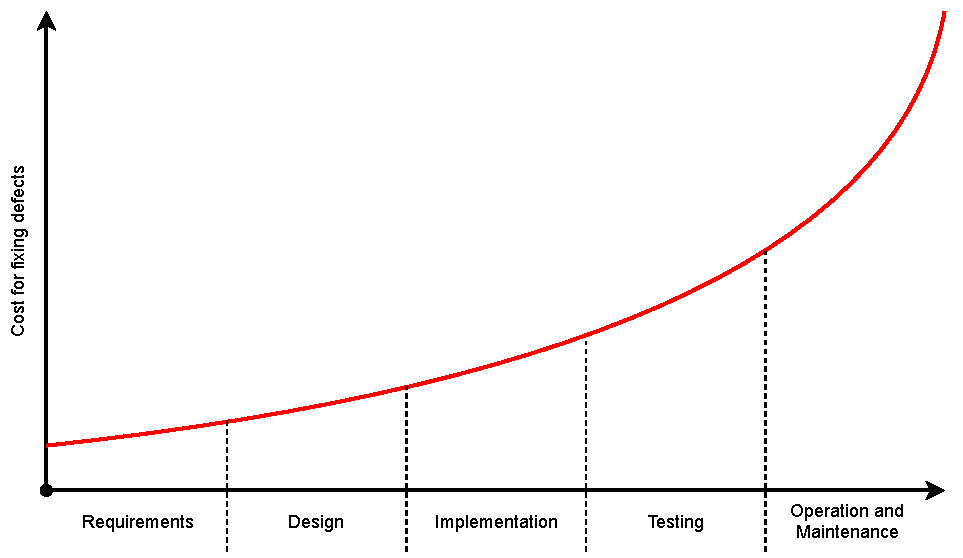
\includegraphics[width=0.7\textwidth]{Images/Chapter1/Background/Cost_of_fixing_bugs/Cost_of_fixing_bugs.pdf}
    \caption{Cost of fixing software system defects \cite{Ogheneovo2014}}\label{fig:CH1_Costs_of_fixing_bugs}
\end{figure} 

Under most circumstances maintenance is implemented if a software system does not meet the required functions specified by the performance requirements \cite{Ogheneovo2014},\cite{Sneed2004}. These systems will also most likely have multiple software defects or will be extremely complex due to:
\begin{itemize}
    \item \textbf{Problem domain being complex:} The software may not be well defined or structured. This is due how large the software systems grow over its entire life cycle or duplicate software components that are made. This is caused by poor understanding of the system architecture by developers not doing the required maintenance on these systems and just adding new features \cite{Galster2019}, \cite{Booch1986}.
    \item \textbf{Difficulties of managing development process:} Most companies will strife to increase their digital products and services over the life cycle of the software project to maximize possible profits with the resources invested \cite{Niu2018}. Increasing production of the development process will only strain the efforts of maintaining software systems \cite{Sneed2004}.\par The development team needs to prioritize concrete task in the development process to make the project feasible, by just focusing on these task poor decisions are made about the required task to perform software maintenance \cite{Galster2019}, \cite{Ogheneovo2014}, \cite{Lenarduzzi2017}. 
    \item \textbf{Flexibility of the software:} Trying to predict what the possible future architecture may look like and modifying it while preserving the software's integrity, may be difficult in software maintenance \cite{Garlan1999}. Software is flexible if it is adaptable to the problem domain when adding modifications to it \cite{Ogheneovo2014}.\par Most development teams will follow a software development methodology to create a future architecture that is modular and structured to preserve the development integrity of new software \cite{Vijayasarathy2016}, \cite{Rehman2018}. This will also have an impact the maintenance methodology the development team will use which are the called corrective, perfective, adaptive and preventive maintenance \cite{FrancisThamburaj2017}.
    \item \textbf{Change in the user's requirements:} In software development the users will often request new additional requirements to the software systems that are delivered to them \cite{Ogheneovo2014}. Modifying software systems may include new additional features that change the initial system architecture. Maintenance on these systems are crucial to ensure that existing components of the system will work as intended with the new components that are added.
\end{itemize}
\newpage

\subsection{Need for a logging mechanism}
No study was found where both the logging mechanism and analysis were combined.
There is a need to develop a method to implement a user-activity logging
the mechanism to do further analysis of the logs to improve software
maintenance.

\subsection{Objectives of the study}
The goal of the study is to develop a logging mechanism to track user-based
activities to preform analysis of these logs to improve system maintenance in
software environment. The study is divided in two components to achieve the
primary goal which is the design and implementation of the logging mechanism
and the analysis of the system utilisation to improve system maintenance.

\subsubsection{Logging mechanism:}
\begin{itemize}
    \item Random text.
\end{itemize}

\subsubsection{Analysis of the system utilisation to improve software maintenance}
\begin{itemize}
    \item Random text.
\end{itemize}

\subsection{Overview of the dissertation}
\subsubsection{Chapter 1: Introduction}
This chapter contains the background of software maintenance and system
utilisation analysis.
\subsubsection{Chapter 2: Mehtodolgy}

\newpage
\section{Literature Study}

\subsection{Preamble}
Introduction of section.

\subsection{Software Maintenance}

\subsection{Event-based logging}
In this section the event-based logging will be discussed and how it is part of software maintenance. 

\subsection{User-based activities in Web-based applications}
In this section, the user-activities in Web-based applications will be discussed.

\subsection{Logging mechanism development}

\section{Conclusion}

